% !TEX encoding = UTF-8
% !TEX TS-program = pdflatex
% !TEX root = ../../tesi.tex

\section{Pianificazione temporale}
Lo stage si è svolto in una durata pari a 8 settimane, nel periodo che va dal 03-05-2021 al 25-06-2021, per un totale di 320 ore, ovvero 40 ore a settimana. Queste 8 settimane sono state divise in 3 periodi principali: il periodo di formazione, dove ho dovuto studiare i principi alla base delle varie \textit{blockchain} che sono andato ad utilizzare, con i relativi linguaggi di programmazione per la stesura degli \textit{smart contract}; il periodo di sviluppo dove ho dovuto produrre i vari \textit{smart contract} e le relative integrazioni con il \textit{back-end}; il periodo di validazione, collaudo e presentazione del prodotto. \\

\noindent La pianificazione settimanale è la seguente: 
\begin{itemize}
  \item \textbf{Prima settimana (40 ore)}:
  \begin{itemize}
      \item incontro con persone coinvolte nel progetto per discutere i requisiti e le richieste relative al sistema da sviluppare;
      \item verifica credenziali e strumenti di lavoro assegnati;
      \item studio dei concetti generali riguardanti la \textit{blockchain}.
  \end{itemize}
  \item \textbf{Seconda settimana (40 ore)}:
  \begin{itemize}
      \item studio della \textit{blockchain} Ethereum.
  \end{itemize}
  \item \textbf{Terza settimana (40 ore)}:
  \begin{itemize}
      \item studio del linguaggio Solidity per la definizione di \textit{smart contract}.
  \end{itemize}
  \item \textbf{Quarta settimana (40 ore)}:
  \begin{itemize}
      \item studio e implementazione degli \textit{smart contract} per la gestione di NFT seguendo lo standard ERC721 su \textit{blockchain} Ethereum.
  \end{itemize}
  \item \textbf{Quinta settimana (40 ore)}:
  \begin{itemize}
      \item studio della \textit{blockchain} HotMoka.
  \end{itemize}
  \item \textbf{Sesta settimana (40 ore)}:
  \begin{itemize}
      \item studio e implementazione degli \textit{smart contract} per la gestione di NFT seguendo gli standard HotMoka.
  \end{itemize}
  \item \textbf{Settima settimana (40 ore)}:
  \begin{itemize}
      \item conclusione codifica;
      \item integrazione tra il \textit{back-end} e una delle due implementazioni sviluppate;
      \item stesura della documentazione relativa al periodo di codifica.
  \end{itemize}
  \item \textbf{Ottava settimana (40 ore)}:
  \begin{itemize}
      \item collaudo della soluzione e stesura della documentazione finale;
      \item incontro di presentazione della soluzione con gli \textit{stakeholders};
      \item \textit{live demo} del lavoro di stage.
  \end{itemize}
\end{itemize}

\begin{figure}[!h]
  \centering
  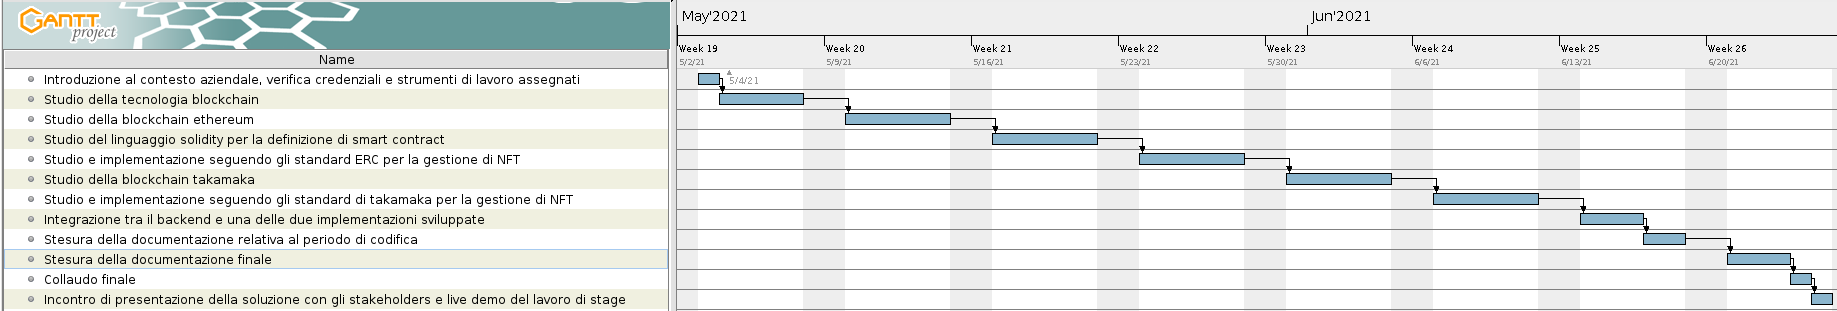
\includegraphics[width=\columnwidth]{capitolo2/gantt.png}
  \caption{Diagramma di Gantt relativo alla pianificazione dello stage}
\end{figure}

Per quanto riguarda la ripartizione oraria delle principali attività, qui si può vedere la tabella riassuntiva:
\begin{longtabu}{|c|X|}
	\hline

  \textbf{Durata in ore} & \textbf{Descrizione dell'attività} \\ \hline
  
	\textbf{160} & \textbf{Studio delle tecnologie} \\
  \textit{40} &
  Studio dei concetti generali riguardanti la \textit{blockchain} \\
  \textit{40} & 
  Studio della \textit{blockchain} Ethereum \\
  \textit{40} & 
  Studio del linguaggio Solidity per la definizione di \textit{smart contract} \\
  \textit{40} & 
  Studio della \textit{blockchain} HotMoka \\

  \hline

  \textbf{80} & \textbf{Implementazione degli \textit{smart contract} per la gestione di NFT} \\ 
  \textit{40} & 
  Studio e implementazione degli \textit{smart contract} per la gestione di NFT seguendo lo standard ERC721 su \textit{blockchain} Ethereum \\
  \textit{40} & 
  Studio e implementazione degli \textit{smart contract} per la gestione di NFT seguendo gli standard HotMoka \\
  
  \hline
  
  \textbf{24} & \textbf{Integrazione tra il backend e una delle due implementazioni sviluppate} \\
  \hline

  \textbf{40} & \textbf{Stesura documentazione} \\ 
  \textit{16} & 
  Stesura della documentazione relativa al periodo di codifica \\
  \textit{24} & 
  Stesura della documentazione finale \\

  \hline

  \textbf{16} & \textbf{Collaudo Finale}  \\ 
  \textit{13} & 
  Collaudo \\
  \textit{1} &
  Incontro di presentazione della piattaforma con gli \textit{stakeholders} \\
  \textit{2} & 
  Live demo del lavoro di stage \\
  \hline

  \textbf{Totale ore} & \multicolumn{1}{c}{\textbf{320}} \\ \hline

  \caption{Tabella riassuntiva delle ore per attività}
\end{longtabu}
